\documentclass[11pt,a4paper]{article}
\usepackage[utf8]{inputenc}
\usepackage[T1]{fontenc}
\usepackage{babel}
\babelprovide[import,main]{spanish}
\renewcommand{\tablename}{Tabla}
\usepackage[margin=2.3cm]{geometry}
\usepackage{amsmath,amssymb,graphicx,booktabs,longtable,array,xcolor,hyperref,needspace,float}
\let\originalsection\section
\renewcommand{\section}{\Needspace{.42\textheight}\originalsection}
\definecolor{azul}{RGB}{0,73,118}
\hypersetup{colorlinks=true,linkcolor=azul,urlcolor=azul,citecolor=azul}
\setlength{\parskip}{5pt}
\setlength{\parindent}{0pt}
\setlength{\emergencystretch}{3em}
\title{\color{azul}Análisis estadístico comparado de cinco ventanas temporales}
\author{Oriana Giraldo Arcia \and Luis Javier Rubio Hernández}
\date{Proyecto Aplicado de Ciencia de Datos, PUJ Cali\\Revisión técnica: 10 de septiembre de 2026}
\begin{document}
\renewcommand{\tablename}{Tabla}
\maketitle
\section{Propósito y alcance estadístico}
El análisis examina la distribución y las asociaciones de los indicadores construidos en los cortes 7, 14, 28, 42 y 56. Corresponde a una exploración previa al modelado: se analizan todos los datos elegibles y no se atribuyen a estos resultados propiedades de validación predictiva. Cada corte mantiene su propia población en riesgo y su evento futuro hasta el final de la presentación.

Se describen cuantiles, dispersión, faltantes y valores extremos. Los faltantes estructurales se separan de valores cero: no existe recencia definida sin actividad ni proporción de cumplimiento observable sin evaluaciones programadas. Los diagnósticos de valores atípicos mediante rango intercuartílico y desviación absoluta mediana no eliminan registros; cuando la escala es cero, el diagnóstico respectivo se conserva como no definido. Los patrones observados no demuestran mecanismos MAR o MNAR.

\section{Asociaciones e incertidumbre dentro de cada corte}
La comparación numérica usa el efecto biserial por rangos, calculado a partir del estadístico de Mann--Whitney con tratamiento de empates \cite{revscipy}:
\[
r_{rb}=\frac{2U_1}{n_1n_0}-1.
\]
El grupo 1 corresponde al retiro futuro. Un efecto negativo indica valores generalmente menores en ese grupo y un efecto positivo indica valores mayores. Para cada indicador se utilizan los casos observables de ambos grupos; por ello, algunos denominadores cambian incluso dentro de un mismo corte. Las estimaciones no son efectos causales ni medidas del rendimiento de un clasificador.

Los intervalos puntuales del 95 por ciento se obtienen mediante 5\,000 remuestreos de personas con reposición, conservando conjuntamente sus inscripciones dentro del corte; se utiliza la semilla 20260908. Esta construcción reconoce la agrupación por estudiante \cite{revfield2007}. Las presentaciones observadas permanecen fijas y no se incorpora incertidumbre por muestreo de cursos. Los intervalos son exploratorios, no simultáneos: no se presentan pruebas de significancia múltiples ni se usa su solapamiento como contraste entre ventanas.

\Needspace{0.42\textheight}
\begingroup\small\setlength{\tabcolsep}{3pt}\renewcommand{\arraystretch}{1.16}
\begin{longtable}{>{\raggedright\arraybackslash}p{0.3375\linewidth}>{\raggedright\arraybackslash}p{0.1125\linewidth}>{\raggedright\arraybackslash}p{0.1125\linewidth}>{\raggedright\arraybackslash}p{0.1125\linewidth}>{\raggedright\arraybackslash}p{0.1125\linewidth}>{\raggedright\arraybackslash}p{0.1125\linewidth}}
\caption{Efecto biserial por rangos en cada corte; no aplica indica ausencia de observaciones suficientes.}\label{multi03:efectos}\\
\toprule
\textbf{Indicador} & \textbf{7} & \textbf{14} & \textbf{28} & \textbf{42} & \textbf{56} \\
\midrule\endfirsthead
\toprule
\textbf{Indicador} & \textbf{7} & \textbf{14} & \textbf{28} & \textbf{42} & \textbf{56} \\
\midrule\endhead
\bottomrule\endfoot
Clics acumulados & -0,179 & -0,147 & -0,107 & -0,111 & -0,114 \\*
Proporción de días activos & -0,163 & -0,132 & -0,120 & -0,121 & -0,129 \\*
Recencia relativa & 0,078 & 0,075 & 0,104 & 0,150 & 0,162 \\*
CV de calendario & 0,109 & 0,109 & 0,126 & 0,129 & 0,140 \\*
CV entre días activos & -0,009 & -0,004 & 0,038 & 0,037 & 0,045 \\*
Tendencia de 7 días & No aplica & -0,012 & -0,064 & -0,082 & 0,013 \\*
Tendencia de 14 días & No aplica & No aplica & 0,046 & -0,133 & -0,093 \\*
Entregas acumuladas & -0,017 & -0,064 & -0,062 & -0,065 & -0,130 \\*
Proporción programada entregada & No aplica & -0,118 & -0,135 & -0,140 & -0,200 \\*
\end{longtable}\endgroup
Los clics acumulados y la proporción de días activos presentan asociaciones negativas con el retiro futuro en todos los cortes. El CV de calendario y la recencia relativa presentan asociaciones positivas; el CV entre días activos se evalúa separadamente. La dependencia entre variabilidad y frecuencia impide presentar estas asociaciones como evidencia independiente. Sin embargo, las magnitudes cambian al variar simultáneamente la historia observada, la población y el horizonte; no permiten afirmar que un corte sea superior a otro para predecir.


\begin{figure}[htbp]\centering
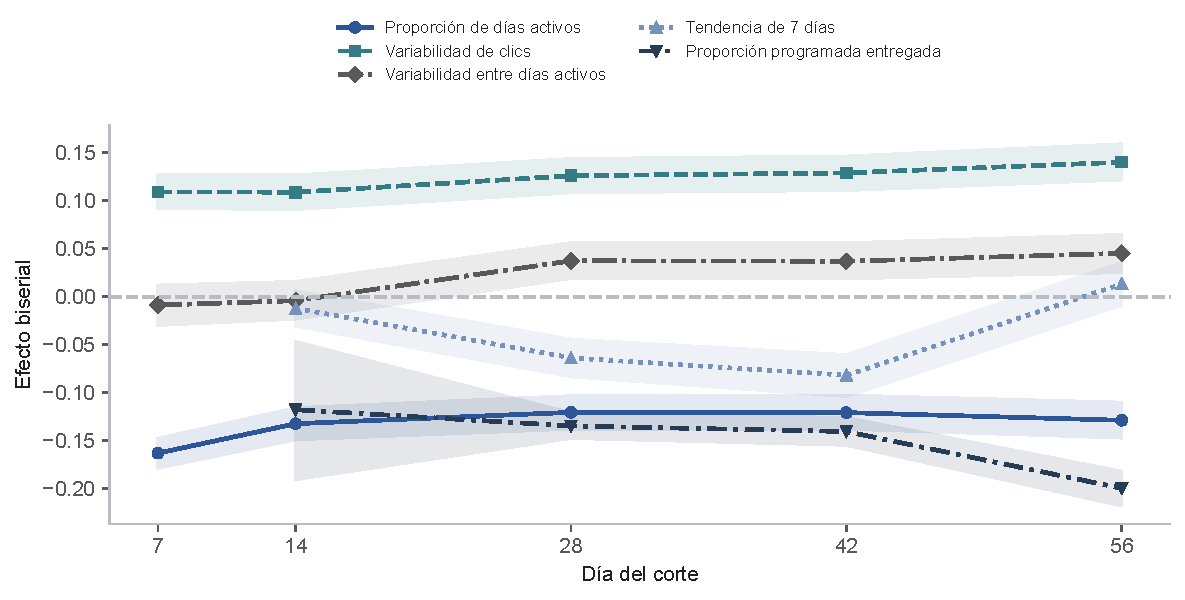
\includegraphics[width=.94\linewidth]{../figuras/03_efectos_cortes.pdf}
\caption{Efectos por corte e intervalos puntuales mediante remuestreo de personas. Las líneas conectan estimaciones y no representan un contraste longitudinal.}\label{multi03:figefectos}\end{figure}
La tendencia de siete días en el corte 56 presenta un efecto de 0,013, con intervalo de -0,009 a 0,036. Este resultado no respalda una dirección clara de asociación para ese indicador en ese corte; tampoco demuestra ausencia de utilidad predictiva conjunta. La tendencia de catorce días conserva un significado distinto porque resume dos bloques de mayor duración.

\section{Disponibilidad, distribución y heterogeneidad}
La comparación de proporciones y recencias relativas reduce la dependencia aritmética de la duración observada, pero no iguala las oportunidades educativas. Las distribuciones empíricas se presentan por corte y las tablas completas conservan los tamaños observados y ausentes. La proporción entregada se analiza solo donde hay evaluaciones programadas; en el día 7 no existe este denominador y no se estima un efecto.


\begin{figure}[htbp]\centering
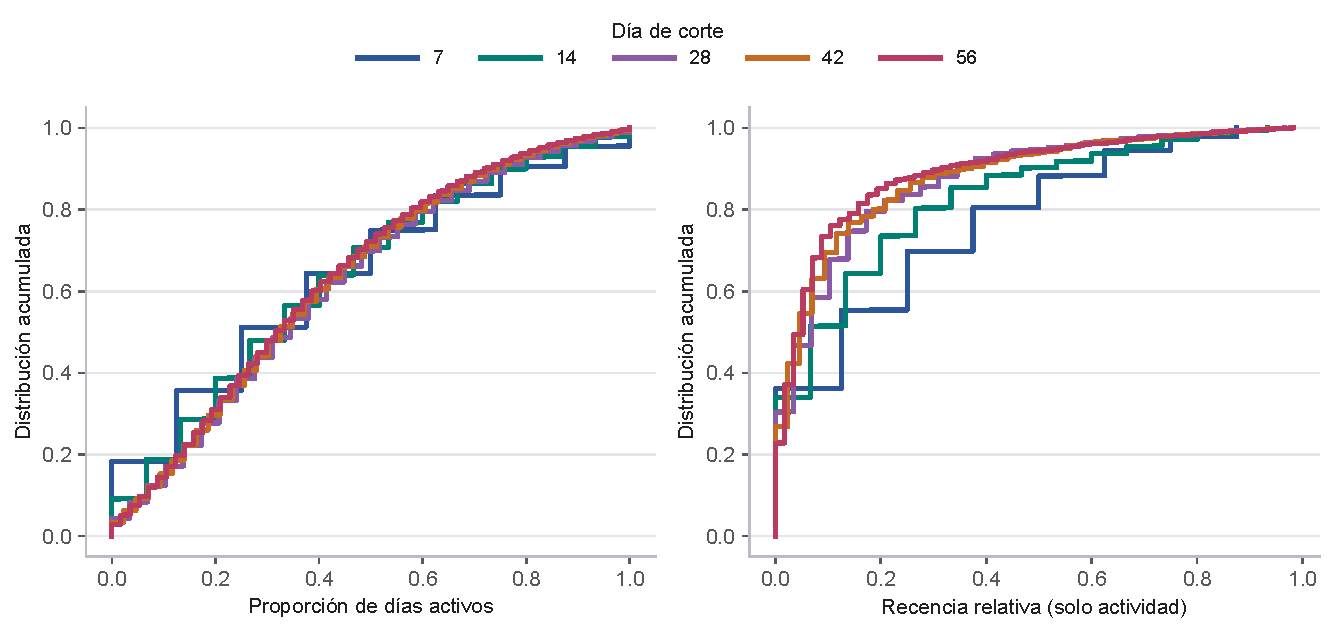
\includegraphics[width=.94\linewidth]{../figuras/03_distribuciones_cortes.pdf}
\caption{Distribuciones acumuladas de actividad relativa y recencia relativa; esta última excluye inscripciones sin actividad observable.}\label{multi03:distribuciones}\end{figure}
La V de Cramér se calcula como $V=\sqrt{\chi^2/[N\min(f-1,g-1)]}$, donde $N$ es el total de la tabla de contingencia y $f,g$ sus dimensiones. Se utiliza como medida descriptiva de asociación, sin atribuir a su valor significancia estadística ni crecimiento necesario por desbalance de categorías.

\Needspace{0.42\textheight}
\begingroup\small\setlength{\tabcolsep}{3pt}\renewcommand{\arraystretch}{1.16}
\begin{longtable}{>{\raggedright\arraybackslash}p{0.29690721649484536\linewidth}>{\raggedright\arraybackslash}p{0.12061855670103093\linewidth}>{\raggedright\arraybackslash}p{0.12061855670103093\linewidth}>{\raggedright\arraybackslash}p{0.12061855670103093\linewidth}>{\raggedright\arraybackslash}p{0.12061855670103093\linewidth}>{\raggedright\arraybackslash}p{0.12061855670103093\linewidth}}
\caption{V de Cramér descriptiva; sin interpretación causal ni pruebas por filas independientes.}\label{multi03:categorias}\\
\toprule
\textbf{Categoría} & \textbf{7} & \textbf{14} & \textbf{28} & \textbf{42} & \textbf{56} \\
\midrule\endfirsthead
\toprule
\textbf{Categoría} & \textbf{7} & \textbf{14} & \textbf{28} & \textbf{42} & \textbf{56} \\
\midrule\endhead
\bottomrule\endfoot
Edad & 0,026 & 0,016 & 0,012 & 0,011 & 0,011 \\*
Módulo & 0,173 & 0,170 & 0,159 & 0,144 & 0,137 \\*
Presentación & 0,082 & 0,059 & 0,043 & 0,040 & 0,033 \\*
Discapacidad & 0,061 & 0,065 & 0,065 & 0,065 & 0,064 \\*
Género & 0,035 & 0,029 & 0,029 & 0,025 & 0,024 \\*
Educación previa & 0,071 & 0,057 & 0,051 & 0,045 & 0,038 \\*
Privación (IMD) & 0,073 & 0,055 & 0,049 & 0,052 & 0,051 \\*
Región & 0,043 & 0,026 & 0,026 & 0,027 & 0,029 \\*
\end{longtable}\endgroup
La asociación con el módulo evidencia heterogeneidad contextual que debe considerarse al diseñar la validación. La V de Cramér no indica una dirección del efecto ni ajusta por otros atributos. Las tasas por nivel y los conteos se exportan por separado; no se interpreta una diferencia descriptiva como efecto atribuible a una característica personal.

\section{Redundancia y estructura multivariada}
Se calculan correlaciones de Spearman y cantidades de pares observados para cada corte. El diagnóstico VIF usa un conjunto reducido de cuatro indicadores con intercepto; sus valores describen dependencia lineal en ese conjunto y no ordenan automáticamente las variables por utilidad. La relación entre volumen de clics, días activos y filas VLE exige evitar interpretaciones de contribuciones completamente independientes.

El análisis de componentes principales utiliza cinco indicadores conductuales: logaritmo de uno más el volumen, proporción de días activos, logaritmo de uno más el promedio por día activo, recencia relativa y coeficiente de variación. Se restringe a casos con actividad y datos completos; cada corte se estandariza y ajusta separadamente \cite{revpca}. Por ello, sus componentes no constituyen un sistema de ejes común para seguir trayectorias individuales entre ventanas.

\Needspace{0.3\textheight}
\begingroup\small\setlength{\tabcolsep}{3pt}\renewcommand{\arraystretch}{1.16}
\begin{longtable}{>{\raggedright\arraybackslash}p{0.13\linewidth}>{\raggedright\arraybackslash}p{0.29\linewidth}>{\raggedright\arraybackslash}p{0.5\linewidth}}
\caption{Resumen descriptivo del PCA ajustado separadamente por corte.}\label{multi03:pca}\\
\toprule
\textbf{Corte} & \textbf{Casos observados} & \textbf{Varianza de dos componentes (\%)} \\
\midrule\endfirsthead
\toprule
\textbf{Corte} & \textbf{Casos observados} & \textbf{Varianza de dos componentes (\%)} \\
\midrule\endhead
\bottomrule\endfoot
7 & 23\,760 & 88,10 \\*
14 & 25\,503 & 87,20 \\*
28 & 26\,312 & 87,24 \\*
42 & 26\,087 & 87,57 \\*
56 & 25\,741 & 87,10 \\*
\end{longtable}\endgroup
La covarianza robusta mediante MCD se ajusta sobre una muestra reproducible de 5\,000 casos por corte y evalúa distancias en los casos completos \cite{revmcd}. La bandera usa el percentil empírico 97,5 de las distancias de todos los casos evaluados en ese corte. Este umbral es descriptivo, no una probabilidad calibrada de anomalía; no se utiliza una prueba de Hotelling ni se eliminan las observaciones marcadas. Las cargas de PCA, VIF y resúmenes MCD permanecen disponibles en CSV.

\section{Sensibilidad con población y evento comunes}
La intersección de las poblaciones elegibles contiene 26\,429 inscripciones. Se fija para ellas el evento de retiro posterior al día 56 y hasta el final, con 3\,985 eventos, y se describen nuevamente cinco indicadores en cada corte. Esta comparación mantiene población y etiqueta; los denominadores observables todavía cambian cuando un indicador requiere actividad o evaluaciones programadas.

\Needspace{0.3\textheight}
\begingroup\small\setlength{\tabcolsep}{3pt}\renewcommand{\arraystretch}{1.16}
\begin{longtable}{>{\raggedright\arraybackslash}p{0.3375\linewidth}>{\raggedright\arraybackslash}p{0.1125\linewidth}>{\raggedright\arraybackslash}p{0.1125\linewidth}>{\raggedright\arraybackslash}p{0.1125\linewidth}>{\raggedright\arraybackslash}p{0.1125\linewidth}>{\raggedright\arraybackslash}p{0.1125\linewidth}}
\caption{Efectos descriptivos en la cohorte común, sin intervalos ni contraste entre cortes.}\label{multi03:comun}\\
\toprule
\textbf{Indicador} & \textbf{7} & \textbf{14} & \textbf{28} & \textbf{42} & \textbf{56} \\
\midrule\endfirsthead
\toprule
\textbf{Indicador} & \textbf{7} & \textbf{14} & \textbf{28} & \textbf{42} & \textbf{56} \\
\midrule\endhead
\bottomrule\endfoot
CV de calendario & 0,067 & 0,082 & 0,103 & 0,114 & 0,140 \\*
CV entre días activos & -0,011 & 0,000 & 0,040 & 0,044 & 0,046 \\*
Tendencia de 7 días & No aplica & -0,010 & -0,042 & -0,074 & 0,013 \\*
Proporción de días activos & -0,074 & -0,087 & -0,089 & -0,102 & -0,128 \\*
Proporción programada entregada & No aplica & -0,097 & -0,101 & -0,118 & -0,199 \\*
\end{longtable}\endgroup
La selección exige conocer que una inscripción permanece elegible hasta el día 56. En consecuencia, es retrospectiva y condicionada a supervivencia administrativa; no puede utilizarse como población operativa de una alerta del día 7. La diferencia respecto de las asociaciones principales ayuda a reconocer el papel de la composición, pero no identifica causalmente su contribución ni permite atribuir a la duración de la ventana todo el cambio observado.

\section{Resultados ampliados de las variables de contexto}
Las categorías se analizan en las mismas poblaciones de cada corte. La Tabla~\ref{corr:niveles} publica conteos y tasas por nivel; la categoría No disponible preserva los faltantes de IMD. Los resultados no se interpretan como efectos causales ni como una evaluación exhaustiva de equidad.
\Needspace{0.42\textheight}
\begingroup\small\setlength{\tabcolsep}{3pt}\renewcommand{\arraystretch}{1.16}
\begin{longtable}{>{\raggedright\arraybackslash}p{0.0782608695652174\linewidth}>{\raggedright\arraybackslash}p{0.1858695652173913\linewidth}>{\raggedright\arraybackslash}p{0.13695652173913045\linewidth}>{\raggedright\arraybackslash}p{0.11739130434782608\linewidth}>{\raggedright\arraybackslash}p{0.11739130434782608\linewidth}>{\raggedright\arraybackslash}p{0.14673913043478262\linewidth}>{\raggedright\arraybackslash}p{0.11739130434782608\linewidth}}
\caption{Distribución y asociación de créditos e intentos previos; efecto biserial por rangos.}\label{corr:numericos}\\
\toprule
\textbf{Corte} & \textbf{Variable} & \textbf{Observados} & \textbf{Ausentes} & \textbf{Mediana} & \textbf{Q25--Q75} & \textbf{Efecto} \\
\midrule\endfirsthead
\toprule
\textbf{Corte} & \textbf{Variable} & \textbf{Observados} & \textbf{Ausentes} & \textbf{Mediana} & \textbf{Q25--Q75} & \textbf{Efecto} \\
\midrule\endhead
\bottomrule\endfoot
7 & Créditos & 29\,076 & 0 & 60,000 & 60--90 & 0,165 \\*
7 & Intentos previos & 29\,076 & 0 & 0,000 & 0--0 & 0,028 \\*
14 & Créditos & 28\,054 & 0 & 60,000 & 60--90 & 0,138 \\*
14 & Intentos previos & 28\,054 & 0 & 0,000 & 0--0 & 0,030 \\*
28 & Créditos & 27\,515 & 0 & 60,000 & 60--90 & 0,131 \\*
28 & Intentos previos & 27\,515 & 0 & 0,000 & 0--0 & 0,033 \\*
42 & Créditos & 27\,005 & 0 & 60,000 & 60--90 & 0,125 \\*
42 & Intentos previos & 27\,005 & 0 & 0,000 & 0--0 & 0,036 \\*
56 & Créditos & 26\,506 & 0 & 60,000 & 60--90 & 0,119 \\*
56 & Intentos previos & 26\,506 & 0 & 0,000 & 0--0 & 0,038 \\*
\end{longtable}\endgroup
Los créditos representan la carga registrada y los intentos previos describen antecedentes de inscripción. Sus asociaciones no permiten distinguir mecanismos educativos ni efectos de modificar la carga. Se mantienen como contexto condicionado, sin incorporarlos automáticamente al conjunto de predictores conductuales.
\Needspace{0.2\textheight}
\begingroup\small\setlength{\tabcolsep}{3pt}\renewcommand{\arraystretch}{1.16}
\begin{longtable}{>{\raggedright\arraybackslash}p{0.225\linewidth}>{\raggedright\arraybackslash}p{0.135\linewidth}>{\raggedright\arraybackslash}p{0.135\linewidth}>{\raggedright\arraybackslash}p{0.135\linewidth}>{\raggedright\arraybackslash}p{0.135\linewidth}>{\raggedright\arraybackslash}p{0.135\linewidth}}
\caption{Retiros futuros / inscripciones elegibles (porcentaje) por nivel y corte.}\label{corr:niveles}\\
\toprule
\textbf{Nivel} & \textbf{7} & \textbf{14} & \textbf{28} & \textbf{42} & \textbf{56} \\
\midrule\endfirsthead
\toprule
\textbf{Nivel} & \textbf{7} & \textbf{14} & \textbf{28} & \textbf{42} & \textbf{56} \\
\midrule\endhead
\bottomrule\endfoot
Edad / 0-35 & 4\,796/20\,383 (23,5\%) & 3\,973/19\,575 (20,3\%) & 3\,550/19\,166 (18,5\%) & 3\,184/18\,800 (16,9\%) & 2\,825/18\,443 (15,3\%) \\
Edad / 35-55 & 1\,796/8\,491 (21,2\%) & 1\,571/8\,281 (19,0\%) & 1\,431/8\,156 (17,5\%) & 1\,288/8\,015 (16,1\%) & 1\,150/7\,878 (14,6\%) \\
Edad / 55<= & 40/202 (19,8\%) & 36/198 (18,2\%) & 31/193 (16,1\%) & 28/190 (14,7\%) & 23/185 (12,4\%) \\
Discapacidad / N & 5\,780/26\,298 (22,0\%) & 4\,833/25\,379 (19,0\%) & 4\,335/24\,908 (17,4\%) & 3\,886/24\,461 (15,9\%) & 3\,447/24\,025 (14,3\%) \\
Discapacidad / Y & 852/2\,778 (30,7\%) & 747/2\,675 (27,9\%) & 677/2\,607 (26,0\%) & 614/2\,544 (24,1\%) & 551/2\,481 (22,2\%) \\
IMD / 0-10\% & 773/2\,855 (27,1\%) & 622/2\,706 (23,0\%) & 560/2\,646 (21,2\%) & 514/2\,601 (19,8\%) & 458/2\,545 (18,0\%) \\
IMD / 10-20 & 765/3\,042 (25,1\%) & 610/2\,890 (21,1\%) & 541/2\,823 (19,2\%) & 495/2\,777 (17,8\%) & 443/2\,725 (16,3\%) \\
IMD / 20-30\% & 881/3\,217 (27,4\%) & 723/3\,060 (23,6\%) & 640/2\,979 (21,5\%) & 581/2\,920 (19,9\%) & 522/2\,861 (18,2\%) \\
IMD / 30-40\% & 733/3\,177 (23,1\%) & 604/3\,055 (19,8\%) & 541/2\,997 (18,1\%) & 483/2\,939 (16,4\%) & 425/2\,882 (14,7\%) \\
IMD / 40-50\% & 671/2\,886 (23,3\%) & 554/2\,773 (20,0\%) & 493/2\,714 (18,2\%) & 432/2\,653 (16,3\%) & 389/2\,611 (14,9\%) \\
IMD / 50-60\% & 590/2\,810 (21,0\%) & 515/2\,739 (18,8\%) & 462/2\,688 (17,2\%) & 409/2\,635 (15,5\%) & 362/2\,588 (14,0\%) \\
IMD / 60-70\% & 598/2\,640 (22,7\%) & 513/2\,559 (20,0\%) & 458/2\,509 (18,3\%) & 416/2\,467 (16,9\%) & 366/2\,417 (15,1\%) \\
IMD / 70-80\% & 526/2\,608 (20,2\%) & 464/2\,549 (18,2\%) & 426/2\,515 (16,9\%) & 378/2\,468 (15,3\%) & 328/2\,418 (13,6\%) \\
IMD / 80-90\% & 495/2\,485 (19,9\%) & 428/2\,418 (17,7\%) & 385/2\,377 (16,2\%) & 340/2\,332 (14,6\%) & 304/2\,297 (13,2\%) \\
IMD / 90-100\% & 428/2\,312 (18,5\%) & 383/2\,268 (16,9\%) & 354/2\,240 (15,8\%) & 314/2\,200 (14,3\%) & 279/2\,165 (12,9\%) \\
IMD / No disponible & 172/1\,044 (16,5\%) & 164/1\,037 (15,8\%) & 152/1\,027 (14,8\%) & 138/1\,013 (13,6\%) & 122/997 (12,2\%) \\
Región / East Anglian Region & 633/2\,962 (21,4\%) & 521/2\,851 (18,3\%) & 469/2\,803 (16,7\%) & 418/2\,752 (15,2\%) & 370/2\,707 (13,7\%) \\
Región / East Midlands Region & 510/2\,059 (24,8\%) & 416/1\,966 (21,2\%) & 372/1\,922 (19,4\%) & 339/1\,889 (17,9\%) & 299/1\,849 (16,2\%) \\
Región / Ireland & 221/1\,111 (19,9\%) & 214/1\,114 (19,2\%) & 192/1\,105 (17,4\%) & 172/1\,085 (15,9\%) & 156/1\,069 (14,6\%) \\
Región / London Region & 705/2\,815 (25,0\%) & 523/2\,635 (19,8\%) & 460/2\,572 (17,9\%) & 420/2\,532 (16,6\%) & 381/2\,493 (15,3\%) \\
Región / North Region & 386/1\,629 (23,7\%) & 322/1\,567 (20,5\%) & 283/1\,530 (18,5\%) & 262/1\,509 (17,4\%) & 231/1\,478 (15,6\%) \\
Región / North Western Region & 606/2\,479 (24,4\%) & 513/2\,390 (21,5\%) & 452/2\,331 (19,4\%) & 398/2\,277 (17,5\%) & 340/2\,219 (15,3\%) \\
Región / Scotland & 655/3\,202 (20,5\%) & 644/3\,192 (20,2\%) & 610/3\,160 (19,3\%) & 558/3\,108 (18,0\%) & 509/3\,059 (16,6\%) \\
Región / South East Region & 410/1\,872 (21,9\%) & 337/1\,799 (18,7\%) & 303/1\,767 (17,1\%) & 264/1\,729 (15,3\%) & 234/1\,699 (13,8\%) \\
Región / South Region & 586/2\,758 (21,2\%) & 501/2\,674 (18,7\%) & 447/2\,622 (17,0\%) & 401/2\,576 (15,6\%) & 350/2\,525 (13,9\%) \\
Región / South West Region & 512/2\,193 (23,3\%) & 411/2\,093 (19,6\%) & 369/2\,051 (18,0\%) & 335/2\,017 (16,6\%) & 310/1\,992 (15,6\%) \\
Región / Wales & 418/1\,983 (21,1\%) & 378/1\,944 (19,4\%) & 343/1\,910 (18,0\%) & 310/1\,877 (16,5\%) & 275/1\,842 (14,9\%) \\
Región / West Midlands Region & 568/2\,238 (25,4\%) & 459/2\,133 (21,5\%) & 413/2\,088 (19,8\%) & 362/2\,037 (17,8\%) & 325/2\,000 (16,2\%) \\
Región / Yorkshire Region & 422/1\,775 (23,8\%) & 341/1\,696 (20,1\%) & 299/1\,654 (18,1\%) & 261/1\,617 (16,1\%) & 218/1\,574 (13,9\%) \\
\end{longtable}\endgroup
\section{VIF publicado y decisión sobre el conteo de filas}
\Needspace{0.3\textheight}
\begingroup\small\setlength{\tabcolsep}{3pt}\renewcommand{\arraystretch}{1.16}
\begin{longtable}{>{\raggedright\arraybackslash}p{0.08617021276595743\linewidth}>{\raggedright\arraybackslash}p{0.17234042553191486\linewidth}>{\raggedright\arraybackslash}p{0.15319148936170213\linewidth}>{\raggedright\arraybackslash}p{0.18191489361702126\linewidth}>{\raggedright\arraybackslash}p{0.15319148936170213\linewidth}>{\raggedright\arraybackslash}p{0.15319148936170213\linewidth}}
\caption{VIF con intercepto en la especificación de auditoría de cuatro indicadores.}\label{corr:vif}\\
\toprule
\textbf{Corte} & \textbf{n} & \textbf{Clics} & \textbf{Proporción activa} & \textbf{Filas VLE} & \textbf{Entregas} \\
\midrule\endfirsthead
\toprule
\textbf{Corte} & \textbf{n} & \textbf{Clics} & \textbf{Proporción activa} & \textbf{Filas VLE} & \textbf{Entregas} \\
\midrule\endhead
\bottomrule\endfoot
7 & 29\,076 & 3,707 & 3,388 & 6,656 & 1,052 \\*
14 & 28\,054 & 4,452 & 4,045 & 8,495 & 1,049 \\*
28 & 27\,515 & 5,235 & 4,696 & 10,929 & 1,319 \\*
42 & 27\,005 & 5,839 & 5,372 & 12,334 & 1,323 \\*
56 & 26\,506 & 6,157 & 5,673 & 13,694 & 1,394 \\*
\end{longtable}\endgroup
El mayor VIF corresponde al conteo de filas en cada corte y llega a 10,929 al día 28. Se conserva esta especificación como diagnóstico de la decisión de exclusión; no es el conjunto predictivo final. La redundancia y la procedencia no resuelta del conteo se consideran conjuntamente, sin imponer un umbral universal para todos los modelos.
\section{Sensibilidad de variabilidad y componentes principales}
\Needspace{0.3\textheight}
\begingroup\small\setlength{\tabcolsep}{3pt}\renewcommand{\arraystretch}{1.16}
\begin{longtable}{>{\raggedright\arraybackslash}p{0.09574468085106384\linewidth}>{\raggedright\arraybackslash}p{0.2297872340425532\linewidth}>{\raggedright\arraybackslash}p{0.22021276595744685\linewidth}>{\raggedright\arraybackslash}p{0.1819148936170213\linewidth}>{\raggedright\arraybackslash}p{0.17234042553191492\linewidth}}
\caption{Correlación con proporción activa en los mismos casos con al menos dos días activos.}\label{corr:cv}\\
\toprule
\textbf{Corte} & \textbf{CV calendario observable} & \textbf{CV activo observable} & \textbf{Rho calendario} & \textbf{Rho activo} \\
\midrule\endfirsthead
\toprule
\textbf{Corte} & \textbf{CV calendario observable} & \textbf{CV activo observable} & \textbf{Rho calendario} & \textbf{Rho activo} \\
\midrule\endhead
\bottomrule\endfoot
7 & 23\,760 & 18\,704 & -0,848 & 0,126 \\*
14 & 25\,503 & 22\,779 & -0,892 & 0,153 \\*
28 & 26\,312 & 25\,227 & -0,909 & 0,102 \\*
42 & 26\,087 & 25\,323 & -0,918 & 0,102 \\*
56 & 25\,741 & 25\,147 & -0,926 & 0,076 \\*
\end{longtable}\endgroup
El CV activo separa mejor la dispersión de intensidad de la frecuencia en estos datos, a costa de una menor observabilidad. No se identifica independencia estadística ni ganancia predictiva. El CV de calendario combina ambos componentes y no se descarta retrospectivamente como cálculo erróneo.
En los cortes 7 y 14, los intervalos puntuales del CV activo incluyen cero y no respaldan una dirección clara. Esta diferencia respecto del CV de calendario muestra que cambiar la definición modifica la interpretación del indicador; no prueba ausencia de utilidad conjunta en un clasificador.
\Needspace{0.3\textheight}
\begingroup\small\setlength{\tabcolsep}{3pt}\renewcommand{\arraystretch}{1.16}
\begin{longtable}{>{\raggedright\arraybackslash}p{0.09574468085106384\linewidth}>{\raggedright\arraybackslash}p{0.1819148936170213\linewidth}>{\raggedright\arraybackslash}p{0.22021276595744685\linewidth}>{\raggedright\arraybackslash}p{0.22021276595744685\linewidth}>{\raggedright\arraybackslash}p{0.1819148936170213\linewidth}}
\caption{Varianza porcentual de dos componentes; comparación descriptiva sobre la misma población.}\label{corr:pcasens}\\
\toprule
\textbf{Corte} & \textbf{n común} & \textbf{Original (5)} & \textbf{Sin volumen (4)} & \textbf{CV activo (4)} \\
\midrule\endfirsthead
\toprule
\textbf{Corte} & \textbf{n común} & \textbf{Original (5)} & \textbf{Sin volumen (4)} & \textbf{CV activo (4)} \\
\midrule\endhead
\bottomrule\endfoot
7 & 18\,704 & 84,27 & 80,53 & 68,57 \\*
14 & 22\,779 & 84,73 & 81,25 & 69,00 \\*
28 & 25\,227 & 85,95 & 82,91 & 70,48 \\*
42 & 25\,323 & 86,61 & 83,72 & 70,76 \\*
56 & 25\,147 & 86,34 & 83,41 & 69,77 \\*
\end{longtable}\endgroup
La especificación original incluye logaritmos de volumen e intensidad, proporción activa, recencia relativa y CV de calendario. La segunda retira volumen; la tercera sustituye además el CV por su versión activa. Todas se ajustan separadamente por corte y se estandarizan. Cambiar el número y significado de las variables cambia el total de varianza: un porcentaje mayor no acredita una representación superior ni explica mayor proporción del abandono.
\section{Sensibilidad de asociaciones a los duplicados exactos}
\Needspace{0.42\textheight}
\begingroup\small\setlength{\tabcolsep}{3pt}\renewcommand{\arraystretch}{1.16}
\begin{longtable}{>{\raggedright\arraybackslash}p{0.2709677419354839\linewidth}>{\raggedright\arraybackslash}p{0.12580645161290321\linewidth}>{\raggedright\arraybackslash}p{0.12580645161290321\linewidth}>{\raggedright\arraybackslash}p{0.12580645161290321\linewidth}>{\raggedright\arraybackslash}p{0.12580645161290321\linewidth}>{\raggedright\arraybackslash}p{0.12580645161290321\linewidth}}
\caption{Cambio del efecto biserial al retirar exactos: alternativa menos fuente original.}\label{corr:duplicadosefectos}\\
\toprule
\textbf{Indicador} & \textbf{7} & \textbf{14} & \textbf{28} & \textbf{42} & \textbf{56} \\
\midrule\endfirsthead
\toprule
\textbf{Indicador} & \textbf{7} & \textbf{14} & \textbf{28} & \textbf{42} & \textbf{56} \\
\midrule\endhead
\bottomrule\endfoot
CV calendario & -0,0007 & -0,0001 & 0,0005 & 0,0003 & 0,0009 \\*
CV activo & -0,0024 & -0,0013 & -0,0004 & -0,0003 & 0,0007 \\*
Tendencia 14 & No aplica & No aplica & -0,0002 & 0,0013 & 0,0004 \\*
Tendencia 7 & No aplica & 0,0011 & 0,0005 & 0,0000 & 0,0008 \\*
Proporción activa & 0,0000 & 0,0000 & 0,0000 & 0,0000 & 0,0000 \\*
Recencia & 0,0000 & 0,0000 & 0,0000 & 0,0000 & 0,0000 \\*
Clics & 0,0001 & 0,0007 & 0,0007 & 0,0011 & 0,0014 \\*
\end{longtable}\endgroup
La alternativa elimina repeticiones en todas las columnas de la fuente antes de agregar; conserva población y evento. La actividad original sigue siendo el análisis principal. Estas diferencias cuantifican sensibilidad descriptiva, no identifican cuál registro es verdadero ni prueban robustez de un modelo aún no entrenado.
\section{Estabilidad de los intervalos por remuestreo}
\Needspace{0.3\textheight}
\begingroup\small\setlength{\tabcolsep}{3pt}\renewcommand{\arraystretch}{1.16}
\begin{longtable}{>{\raggedright\arraybackslash}p{0.14\linewidth}>{\raggedright\arraybackslash}p{0.25\linewidth}>{\raggedright\arraybackslash}p{0.29\linewidth}>{\raggedright\arraybackslash}p{0.26\linewidth}}
\caption{Cambio máximo de extremos entre 2.000 y 5.000 remuestreos; comparación numérica, no contraste de hipótesis.}\label{corr:bootstrap}\\
\toprule
\textbf{Corte} & \textbf{Indicadores} & \textbf{Cambio máximo} & \textbf{Dentro de 0,005} \\
\midrule\endfirsthead
\toprule
\textbf{Corte} & \textbf{Indicadores} & \textbf{Cambio máximo} & \textbf{Dentro de 0,005} \\
\midrule\endhead
\bottomrule\endfoot
7 & 11 & 0,0006 & 11 \\*
14 & 13 & 0,0030 & 13 \\*
28 & 14 & 0,0009 & 14 \\*
42 & 14 & 0,0008 & 14 \\*
56 & 14 & 0,0013 & 14 \\*
\end{longtable}\endgroup
Se compararon los primeros 500 y 2\,000 remuestreos con los 5\,000 de la misma secuencia reproducible. Se fijó una tolerancia descriptiva de 0,005 unidades del efecto para comparar extremos. Las secuencias son anidadas: este diagnóstico no demuestra convergencia con semillas independientes ni elimina error Monte Carlo. Los intervalos publicados utilizan 5\,000 remuestreos y permanecen puntuales y exploratorios.

\section{Conclusiones y continuidad}
La comparación documenta que la disponibilidad académica y el significado de los indicadores cambian con el momento de observación. Las señales conductuales conservan asociaciones descriptivas con el retiro, mientras que algunas tendencias recientes presentan resultados menos definidos. La evidencia favorece mantener explícitos los denominadores, el calendario y la historia requerida, en lugar de completar automáticamente con ceros los indicadores no observables.

Los resultados preparan la comparación posterior de modelos, pero no establecen una ventana óptima. Esa decisión requerirá evaluar discriminación, calibración y utilidad de anticipación bajo particiones compatibles y un protocolo fijado antes de seleccionar modelos, umbrales o cortes. La exploración ya realizada sobre la fuente completa debe declararse al evaluar la independencia de una prueba final; no se presenta ningún subconjunto como intacto por el solo hecho de asignarle después ese nombre.


\par\vspace{6pt}
\bibliographystyle{plain}
\bibliography{referencias_revision}
\end{document}
